\documentclass[a4paper,11pt,notitlepage]{article}
\usepackage{amsmath}
\usepackage{amsfonts}
\usepackage{amssymb}
\usepackage[UTF8]{ctex}
\usepackage{graphicx}
\usepackage{color}
\usepackage{changepage}
\usepackage{enumitem}
\usepackage{subfigure}
\usepackage{float}
\usepackage[backend=biber]{biblatex}

\usepackage{titlesec}
\titleformat{\section}{\bfseries\Large}{$\S$\,\thesection}{1em}{}
\titleformat{\subsection}{\bfseries\large}{\Roman{subsection}}{1em}{}
\titleformat{\subsubsection}{\bfseries\normalsize}{\roman{subsubsection}}{1em}{}
\titlespacing*{\subsection}{2em}{2pt}{2pt}
\titlespacing*{\subsubsection}{3em}{2pt}{2pt}
\title{\vspace{-1.5cm} \textbf{\huge{数值分析第一章上机}}\vspace{-1em}}
\author{By 211870125 陈睿硕}
\date{}

\usepackage{geometry}
\geometry{left=2cm,right=2cm,top=2cm,bottom=2cm}

\usepackage{fancyhdr}
\pagestyle{fancy}
\fancyhf{}
\fancyhead[L]{Chapter 1}
\fancyhead[R]{\thepage}
\setlength{\headheight}{14pt}

\usepackage{listings}  % 引入 listings 包
\lstset{                % 定义代码块的样式
    basicstyle=\normalsize\ttfamily, % 设定代码字体大小、样式
    showspaces=false,   % 不显示空格
    showstringspaces=false, % 不显示字符串中的空格
    showtabs=false,     % 不显示制表符
    frame=single,       % 设定代码块边框样式
    rulecolor=\color{black}, % 设定代码块边框颜色
    tabsize=4,          % 设定制表符长度为 4 个字符
    captionpos=t,       % 设定标题位置为底部
    keywordstyle=\bfseries\color{blue}\ttfamily,
    stringstyle=\color{red}\ttfamily,
    commentstyle=\color{green}\ttfamily,
    morecomment=[l][\color{magenta}]{\#},
    framesep=0.5em,
    frameround=tttt,
    breaklines=true,    % 自动换行
    breakatwhitespace=false, % 只在空格分割处换行
    escapeinside={\%*}{*)}   % 允许使用 LaTeX 命令
}
\renewcommand{\lstlistingname}{代码}

\usepackage{hyperref}
\usepackage{cleveref}
\crefname{theorem}{定理}{定理}
\crefname{figure}{图}{图}
\crefname{equation}{式}{式}
\crefname{listing}{代码}{代码}

\begin{document}
\maketitle
\vspace{-1cm}
\thispagestyle{fancy}

\section{问题}
\begin{adjustwidth}{1em}{0pt}
\begin{enumerate}[label=\textbf{Q\arabic*}]
    \item 求计算机的规范化浮点数的上溢值($OFL$)、下溢值($UFL$)和计算机的机器精度($\varepsilon_{mach}$)。\label{Q1}\notag
    \item 编写并测试子程序,计算$y = x - \sin{x}$,使得有效位的丢失最多 1 位。 \label{Q2}\notag
    \item 计算$y_{n} = \int_{0}^{1} x^{n} e^{x} dx\ \ \ (n \geq 0)$。 \label{Q3}\notag
    \item 考虑由
    \begin{equation*}
        \left\{
        \begin{aligned}
        & x_{0}=1\ \ x_{1}=\frac{1}{3}\\
        & x_{n+1}=\frac{13}{3}x_{n}-\frac{4}{3}x_{n-1}\ \ (n\geq1)
        \end{aligned}
        \right.
        \end{equation*}
    归纳定义的实数序列。将初值改为$x_{0}=1$和$x_{1}=4$数值稳定吗? \label{Q4}\notag
\end{enumerate}
\end{adjustwidth}

\section{算法思路}
\subsection{对\ref{Q1}的解答}
问题即求解$-L$(即单精度数最小指数)、$U$(即单精度数最大指数)、$t$(即单精度数精度)。
这是因为利用公式:
\begin{gather}
    OFL = 2^{U} (2 - 2^{-(t-1)}), \label{eq:1.1}\\
    UFL = 2^{-L}, \label{eq:1.2}\\
    \varepsilon_{mach} = 2^{-t}, \label{eq:1.3}
\end{gather}
可以求得问题之解。\\
\indent 下面我们将分四步求解上溢值,下溢值和机器精度。
\subsubsection{求解\texorpdfstring{$t + L$}{}}
\begin{adjustwidth}{1em}{0pt}
\qquad 我们将$a = 1$不断进行"$\div 2$"操作,直到其变为0,记录下操作的次数$count$。\\
\indent 在$a$变为0的前一刻,$a$的数值应该是单精度浮点数的最小正值,即$2^{-L-(t-1)}$。
这是因为非规格数的指数始终默认为$-L$。
从$a = 1$到$a = 2^{-L-(t-1)}$共进行了$L + t - 1$步,故最后当$a$恰变为$0$时,共进行了$t + L$步。
则有:
\begin{equation}
    t + L = count = 150, \label{eq:1.4}  
\end{equation}
\end{adjustwidth}
\subsubsection{求解\texorpdfstring{$t$}{}}
\begin{adjustwidth}{1em}{0pt}
\qquad 我们令$c = 3,d = 1$,然后不断对两者进行“$\times 2 + 1$"操作,直到式 $c - 1 = 2b$ 不成立,
记录下操作的次数,其即为$t - 1$。\\
\indent 这是因为规格数的有效数字不能超过$t$位,一旦超过$t$位便会产生舍入误差。易见每次操作都将$c$、$d$的有效位数增多一位,
当式 $c - 1 = 2b$ 第一次不成立时,$c$的有效数字恰超过$t$位,$d$的有效数字恰为$t$位,故实际上有:
\begin{equation}
    d = (\underbrace{11\cdots\cdots1}_{t\text{个}})_{2} = 2^{t} - 1, \label{eq:1.5}
\end{equation}
此时也正好进行了$t - 1$次操作,如此可求得$t = 24$。
\end{adjustwidth}
\subsubsection{求解上溢值}
\begin{adjustwidth}{1em}{0pt}
\qquad 结合\cref{eq:1.5}改写\cref{eq:1.1}为:
\[
    OFL = 2^{U-t+1} (2^{t} - 1) = 2^{U-t+1} d
\]
故类似于\MakeUppercase{\romannumeral 2}中的方法,我们不断将$d$进行“$\times 2$"操作,直至发生舍入。
记录下舍入前一刻的d的值,即为上溢值$OFL$。求得上溢值$OFL \approx 3.40282 \times 10^{38}$。
\end{adjustwidth}
\subsubsection{求解下溢值及机器精度}
\begin{adjustwidth}{1em}{0pt}
\qquad 由$t = 24$及\cref{eq:1.4}知$L = 150 - t = 126$,利用\cref{eq:1.2}计算得$UFL \approx 1.17549 \times 10^{-38}$。\\
\indent 由\cref{eq:1.3}计算得$\varepsilon_{mach} \approx 5.96046 \times 10^{-8}$
\end{adjustwidth}

\subsection{对\ref{Q2}的解答}
根据精度损失定理,我们可知当$1-\frac{\sin{x}}{x}\geq\frac{1}{2}$时,精度损失不超过一位。故$\left|x\right|\geq2$时,
我们调用python中math库的sin函数直接计算即可。\\
\indent $\left|x\right|\leq2$时,我们对$x-\sin{x}$进行泰勒展开:
\begin{equation}
    x-\sin(x) = \frac{x^3}{3!} - \frac{x^5}{5!} + \frac{x^7}{7!} - \frac{x^9}{9!} + \frac{x^{11}}{11!} - \cdots\notag
\end{equation}
为了保证使用泰勒级数截断近似后不会丢失超过一位,我们研究$x-\sin{x}$泰勒展开的拉格朗日余项:
\begin{equation}
    R_n(x) = \frac{(-1)^{n+1}\cos(\xi)}{(n+1)!}x^{n+1}\notag
\end{equation}
\\我们希望$\left|R_n(x)\right|\leq2^{-24}$,事实上当$n=15$时,有$\left|R_n(x)\right|\leq\frac{2^{15}}{15!}<2^{-24}$。
故$\left|x\right|\geq2$时,我们可以按照如下公式计算:
\begin{equation}
    x-\sin(x) \approx \frac{x^3}{3!} - \frac{x^5}{5!} + \frac{x^7}{7!} - \frac{x^9}{9!} + \frac{x^{11}}{11!} - \frac{x^{13}}{13!}\notag
\end{equation}

\subsection{对\ref{Q3}的解答}
易见$y_{0}=e-1$,故计算$y_{0}$时会发生舍入误差,若按照递推公式直接迭代计算$y_{n}$,这个舍入误差
和每次迭代时计算$e$的舍入误差因多次与远大于一的数相乘而变得十分巨大,导致算法不稳定。\\
\indent 通过分部积分,我们可以得到$y_{n}$的递推公式:
\begin{equation}
    y_{n+1}=e-(n+1)y_{n}\notag
\end{equation}
利用上述递推公式我们可以理论上地算出:
\begin{equation}
    \int_{0}^{1} x^{n}e^{x} dx = (-1)^n n! (e-1) + (-1)^n n! e \sum_{k=1}^{n} (-1)^k \frac{1}{k!} \notag
\end{equation}
\\注意到
\begin{equation}
    e^{-x}-1=\sum_{k=1}^{\infty}\frac{(-x)^k}{k!}=\sum_{k=1}^{n}\frac{(-x)^k}{k!} + R_{n}(x)\notag
\end{equation}
其中,$R_n(x) = \frac{e^{-cx} }{(n+1)!}x^{n+1},c\in(0,1)$。\\
故有
\begin{equation}
    \left|\int_{0}^{1} x^{n}e^{x} dx \right|= \left|(-1)^n n! (e-1) + (-1)^n n! e (e^{-1}-1-R_{n}(1))\right|
    = \frac{e^{1-c}}{(n+1)}
    \leq \frac{e}{n+1}\notag
\end{equation}
故当$n$足够大时(这里我们取界限为$2^{24}$),我们可以认为$y_{n}=0$,并将递推公式改写为:
\begin{equation}
    y_{n}=\frac{e-y_{n+1}}{n+1}\notag
\end{equation}
如此由后向前逆向递推,可以使误差不断乘远小于1的数从而阶乘级缩小。

\subsection{对\ref{Q4}的解答}
使用递推公式及初值可以求得$x_{n}=\frac{1}{3^{n}}$($x_{0}=1\ \ x_{1}=\frac{1}{3}$时),
$x_{n}=4^{n}$($x_{0}=1\ \ x_{1}=4$时)。
使用python程序直接计算即可,但要注意的是应计算$\frac{1}{3^{n}}$而非$\left(\frac{1}{3}\right)^{n}$,
后者会将舍入误差幂次计算,从而增大误差(见附录\cref{lst:1}中的\textbf{test.py})。

\section{结果分析}
\subsection{对\ref{Q1}的分析}
这个方法是通过找出$t$、$U$、$L$的值利用既知公式计算上溢值、下溢值及机器精度的,故和理论分析的上述三值完全相等。
利用C++的char指针打印出所算出的三值的单精度表示,也和我们理论分析的形式无异,故正确性是肯定的。

\subsection{对\ref{Q2}的分析}
我们将算法在python中实现后,在$x=10^{-t},t=0,1,2,\cdots,10$时直接计算和用泰勒展开计算$x-\sin{x}$,得到如下结果:
\begin{figure}[H]
    \centering
    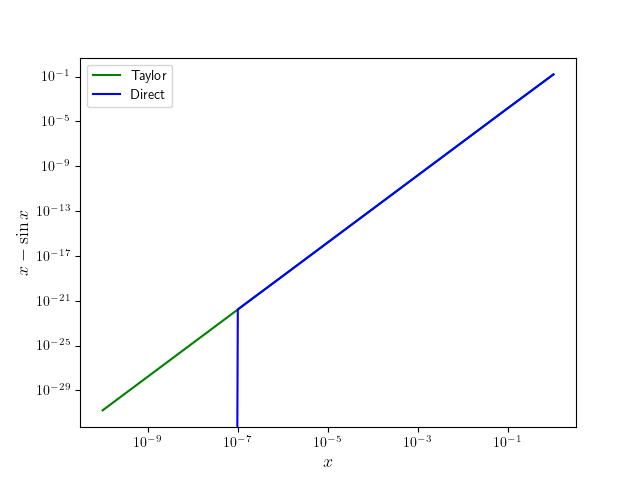
\includegraphics[width=0.8\textwidth]{../picture/Second_Week_1.png}
    \caption{直接计算与用泰勒展开计算结果}
    \label{pic:1}
\end{figure}
\indent 可以看到两种方法的计算结果在$10^{-7}$量级以上极其相近,这也就说明了泰勒展开的近似较为准确。但直接计算的方法在
$10^{-7}$量级以下发生严重偏移,这正是相减相消后精度不够导致的。\\
\indent 并且我们知道$x-\sin{x} \sim O(x^{3})(x\rightarrow0)$,这也和\cref{pic:1}中图像的线性以及直线的斜率相符合。

\subsection{对\ref{Q3}的分析}
考虑到$y_{n}$十分接近$0$,计算的近似值可能会在$0$的上下波动,我们对两种方法计算出的$\left|y_{i}\right|,i=1,2,\cdots,100$作\cref{pic:2}。
\begin{figure}[H]
    \centering
    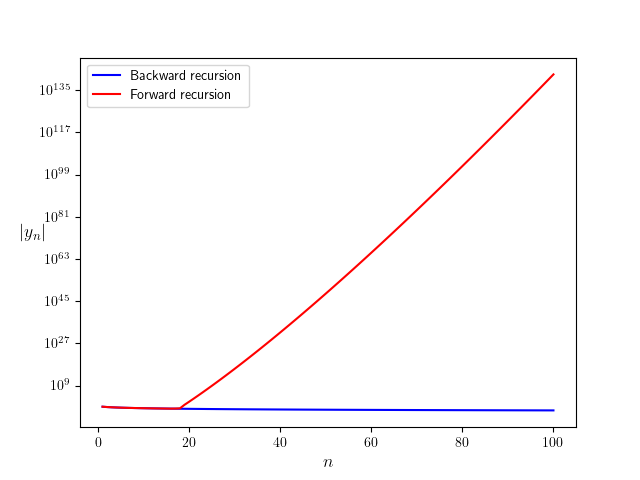
\includegraphics[width=0.8\textwidth]{../picture/Second_Week_2.png}
    \caption{两种递推法算出的$\left|y_{n}\right|$}
    \label{pic:2}
\end{figure}
\indent 可以看到正向递推法求得的$\left|y_{n}\right|$在$n$不较小的情况下表现出了指数级增长,这显然不符合$\left|y_{n}\right|$的单调变化。
而逆向递推法求得的$\left|y_{n}\right|$始终平稳地减小,这是符合实际的。

\subsection{对\ref{Q4}的分析}
利用递推公式迭代计算$x_{n}(n\geq2)$,并计算其与单精度表示的$\frac{1}{3^{n}}$之差,得到\cref{pic:3a}。
\begin{figure}[H]
    \centering
    \subfigure[$x_{n}$与$\frac{1}{3^{n}}$之间的误差]{
    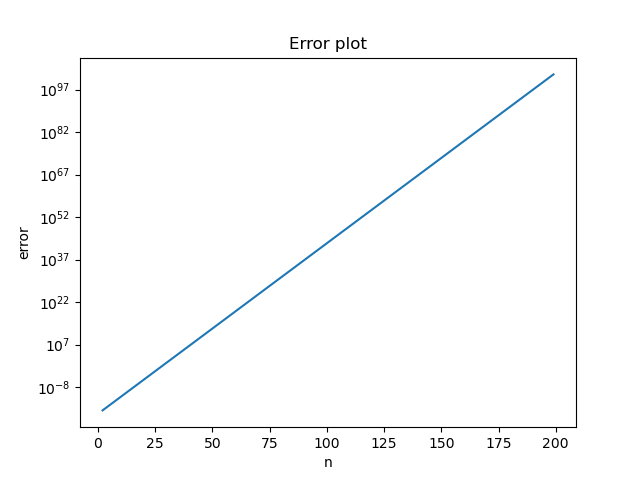
\includegraphics[width=0.45\textwidth]{../picture/Second_Week_3A.png}
    \label{pic:3a}}
    \subfigure[$x_{n}$与$4^{n}$之间的误差]{
    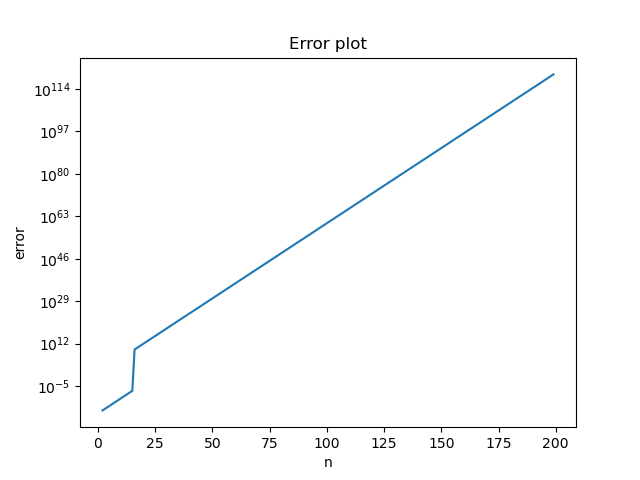
\includegraphics[width=0.45\textwidth]{../picture/Second_Week_3B.png}
    \label{pic:3b}}
    \caption{Q4误差图}
    \label{pic:3}
\end{figure}
\indent 可以看到随着n的增大,误差呈指数型增长,在$n=200$是更是达到了惊人的$10^{97}$量级,说明递推地正向计算是不稳定的。
我们可以发现,误差主要来自于非$3$倍数的整数除以$3$发生的舍入误差在数列的正向递推中不断累积
($\frac{1}{3^{n}}$计算时也发生了舍入误差,但与数列递推产生的误差相比可以忽略不计),我们记
\begin{equation}
    \label{(*)}
    x_{n}=\frac{1}{3^{n}}(1+\varepsilon_{n})
    \tag{\textbf{$*$}}
\end{equation}
记计算$\frac{1}{3}$时产生的舍入误差为$\varepsilon$。易见$\varepsilon_{0}=0$,$\varepsilon_{1}=\varepsilon$。
将(\ref{(*)})式代入递推公式得(事实上递推公式中计算$\frac{13}{3}$与$\frac{4}{3}$也会发生舍入误差,但当$n$不过小时,
此舍入误差的量级远远小于$\varepsilon_{n}$,故在下面的推导中忽略不计):
\begin{equation}
    \varepsilon_{n+1}=13\varepsilon_{n}-12\varepsilon_{n-1}(n\geq1)\notag
\end{equation}
解得$\varepsilon_{n}=\frac{1}{11}(12^{n}-1)\varepsilon$,故可见实际误差(即$x_{n}$与$\frac{1}{3^{n}}$之间的误差)满足:
\begin{equation}
    \widehat{\varepsilon_{n}}=\frac{1}{11}\left[4^{n}-\left(\frac{1}{3}\right)^{n}\right]\varepsilon\approx\frac{4^{n}}{11}\varepsilon \notag
\end{equation}
$\widehat{\varepsilon_{n}}$确实如\cref{pic:3a}关于$n$指数增长。
并且结合Week 1的上机作业可知,$\varepsilon_{mach} \approx 5.96046 \times 10^{-8}$,
$\frac{1}{3}$的舍入误差$\varepsilon$量级上应比$\varepsilon_{mach}$小,
于是$\varepsilon_{2}\approx\frac{16}{11}\varepsilon$的量级小于$10^{-8}$,与\cref{pic:3a}的起始点位置相符合。
\\\indent 类似地,当$x_{0}=1$,$x_{1}=4$时,得到误差图\cref{pic:3b}。
\\\indent 可以看到误差也是呈指数型增长。事实上,若类似上文的定义,应有$\varepsilon_{0}=\varepsilon_{1}=0$,那为何还会发生舍入误差的累积呢?
这是因为其实由于计算$\frac{13}{3}$与$\frac{4}{3}$时发生的舍入误差,$\varepsilon_{2}\neq0$,故同前推导,误差依然会呈指数增长。
但此处与上例不同的是,折线在$n=15$处发生了一次“突变”,我认为这是$\varepsilon_{i}(i=2,3\cdots,15)$
不足以远大于计算$\frac{13}{3}$与$\frac{4}{3}$时发生的舍入误差导致的。

\section{附录:程序代码}
\begin{lstlisting}[language=C++,caption={First Week.cpp}]
#include<iostream>
#include<cmath>
using namespace std;
int main()
{
    float a=1,b=1;
    int t_plus_L=0;
    while(a!=0)
    {
        b=a;
        a/=2;
        t_plus_L++;
    }
    float c=3,d=1,t=1;
    while(c-1==2*d)
    {
        d=2*d+1;
        c=2*c+1;
        t++;
    }
    float u=2*d;
    while(u/2==d)
    {
        u*=2;d*=2;
    }
    cout<<"上溢值为:"<<d<<endl<<"下溢值为:"<<pow(2,t-t_plus_L)<<endl
    <<"机器精度为:"<<pow(2,-t)<<endl;
    return 0;
}
\end{lstlisting}

\begin{lstlisting}[language=Python,caption={Second Week 1.py}]
import math
import matplotlib.pyplot as plt
plt.rcParams['font.sans-serif'] = ['Microsoft YaHei'] 
def calc_y(x):
    if abs(x)>=2:
        y=x-math.sin(x)
        return y
    else:
        rad = x
        return rad**3/6 - rad**5/120 + rad**7/5040 - rad**9/362880 + rad**11/39916800 -rad**13/6227020800
def precise(x):
    return x-math.sin(x)
a = [10**i for i in range(-10,1)][::-1]
b = [calc_y(n) for n in a]
c = [precise(n) for n in a]
plt.plot(a,b,label='使用泰勒级数计算',color='green')
plt.plot(a,c,label='直接计算',color='blue')
plt.xlabel('x')
plt.xscale('log')
plt.yscale('log')
plt.legend()
plt.show()
\end{lstlisting}

\begin{lstlisting}[language=Python,caption={Second Week 2.py}]
import numpy as np
import math
import matplotlib.pyplot as plt
plt.rc('text',usetex=True)
y1=np.zeros(2**24+1)
n=2
for i in list(range(0,2**24))[::-1]:
    y1[i]=(math.e-y1[i+1])/(i+1)
if n>2**24:
    print("y_n=",0)
else:
    print("y_n={:.23f}".format(y1[n]))
y2=np.zeros(101)
y2[0]=math.e-1
for j in range(0,100):
    y2[j+1]=math.e-(j+1)*y2[j]
y2=[abs(k) for k in y2]
fig,ax=plt.subplots()
ax.set_xlabel(r'$n$',fontsize=13)
ax.set_ylabel(r'$\left|y_{n}\right|$',rotation=0,fontsize=13)
ax.plot(range(1,101),y1[1:101],label='Backward recursion',color='blue')
ax.plot(range(1,101),y2[1:101],label='Forward recursion',color='red')
ax.legend()
plt.yscale('log')
plt.show()
\end{lstlisting}

\begin{lstlisting}[language=Python,caption={Second Week 3},label={lst:1}]
##Second_Week_3A.py
import matplotlib.pyplot as plt
import numpy as np
x=np.zeros(200,dtype=float)
x[0]=1
x[1]=1/3
ep=np.zeros(200,dtype=float)
for i in range(2,200):
    x[i]=x[i-1]*13/3-x[i-2]*4/3
    ep[i]=np.abs(1/np.power(3,i)-x[i])
plt.plot(np.arange(2,200), ep[2:200])
plt.xlabel('n')
plt.ylabel('error')
plt.yscale('log')
plt.title('Error plot')
plt.show()

##Second_Week_3B.py
import matplotlib.pyplot as plt
import numpy as np
x=np.zeros(200,dtype=float)
x[0]=1
x[1]=4
ep=np.zeros(200,dtype=float)
for i in range(2,200):
x[i]=x[i-1]*13/3-x[i-2]*4/3
ep[i]=np.abs(np.power(4,i)-x[i])
plt.plot(np.arange(2,200), ep[2:200])
plt.xlabel('n')
plt.ylabel('error')
plt.yscale('log')
plt.title('Error plot')
plt.show()

##test.py
a=float(1/3)**200
b=float(1/3**200)
print(a==b)
\end{lstlisting}

\end{document}
